\section{Basic definitions}





\subsection{Definition and examples for Lie algebras}


\begin{defi}
 Let $\g$ be a vector space over some field $k$. A $k$-bilinear map
 \[
  [\cdot, \cdot] \colon \g \times \g \to \g
 \]
 is called a \emph{Lie bracket} if it satisfies the following two conditions:
 \begin{enumerate}
  \item
   $[\cdot, \cdot]$ is \emph{alternating}, i.e.\ $[x,x] = 0$ for every $x \in \g$.
  \item
   $[\cdot, \cdot]$ satisfies the \emph{Jacobi identity}
   \[
    [x,[y,z]] + [y,[z,x]] + [z,[x,y]] = 0
    \quad
    \text{for all $x,y,z \in \g$}.
   \]
 \end{enumerate}
 A $k$-vector space $\g$ together with the Lie-bracket $[\cdot,\cdot]$ is called a \emph{$k$-Lie algebra}.
\end{defi}


\begin{rem}
 Any Lie bracket $[\cdot, \cdot]$ is antisymmetric, i.e.\ $[y,x] = -[x,y]$ for all $x,y \in \g$, because
 \[
  0 = [x+y, x+y] = [x,x] + [x,y] + [y,x] + [y,y] = [x,y] + [y,x].
 \]
\end{rem}


\begin{rem}
 Using the antisymmetry of the Lie bracket the Jacobi identity can be rewritten as
 \[
  [x,[y,z]] = [[x,y],z] + [y,[x,z]] \quad \text{for all $x,y,z \in \g$}.
 \]
\end{rem}



\begin{expls}
 \begin{enumerate}[leftmargin=*]
  \item
   Any vector space $V$ becomes a Lie algebra via
   \[
    [x,y] = 0 \quad \text{for all $x,y \in V$}.
   \]
  \item
   Any \emph{associative} $k$-algebra $A$ becomes a Lie algebra via
   \[
    [a,b] = ab-ba \quad \text{for all $a,b \in A$}.
   \]
   It is clear that $[\cdot, \cdot]$ is alternating and because $A$ is associative it follows that for all $a,b,c \in A$
   \begin{align*}
    &\, [a,[b,c]] + [b,[c,a]] + [c,[a,b]] \\
    &= [a, (bc-cb)] + [b, (ca-ac)] + [c, (ab-ba)] \\
    &= a(bc-cb)-(bc-cb)a + b(ca-ac) - (ca-ac)b + c(ab-ba) - (ab-ba)c \\
    &= abc -acb -bca +cba +bca -bac -cab +acb +cab -cba -abc +bac \\
    &= 0.
   \end{align*}
   
   The following two are important examples of this construction:
   \begin{enumerate}
    \item
     The $k$-algebra of ($n \times n$)-matrices $\Mat_n(k)$ becomes a Lie algebra via
     \[
      [A,B] = AB-BA \quad \text{for all $A,B \in \Mat_n(k)$}.
     \]
     This is called the \emph{general linear Lie algebra} and is denoted by $\gl_n(k)$.
    \item
     More generally for any $k$-vector space the $k$-algebra $\End_k(V)$ becomes a Lie algebra via
     \[
      [\varphi_1, \varphi_2] \coloneqq \varphi_1 \circ \varphi_2 - \varphi_2 \circ \varphi_1
      \quad
      \text{for all $\varphi_1, \varphi_2 \in \End_k$}.
     \]
     This is called the \emph{general linear Lie algebra for $V$} and is denoted by $\gl(V)$.
   \end{enumerate}
 \end{enumerate}
\end{expls}


\begin{defi}
 Let $\g$ be a $k$-Lie algebra. A \emph{Lie subalgebra} of a $\g$ is a $k$-linear subspace $\h \subseteq \g$ such that
 \[
  [x,y] \in \h \quad \text{for all $x,y \in \h$}.
 \]
 An \emph{ideal} inside $\g$ is a $k$-linear subspace $I \subseteq \g$ such that
 \[
  [x,y] \in I \quad \text{for all $x \in \g$ and $y \in I$}.
 \]
 That $I$ is an ideal in $\g$ is denoted by $I \subideal \g$.
\end{defi}


\begin{rem}
 It is not necessary to distinguish between left ideals or right ideals in a Lie algebra because the Lie bracket is antisymmetric.
\end{rem}


\begin{rem}
 For a Lie algebra $\g$ and a subalgebra $\h \subseteq \g$ it follows that $\h$ becomes a Lie algebra by restricting the Lie bracket of $\g$ to $\h$. Every ideal inside $\g$ is also a subalgebra of $\g$.
\end{rem}


\begin{defi}
 Let $\g$ be a Lie algebra. The \emph{center} of $\g$ is
 \[
  Z(\g) \coloneqq \{x \in \g \mid \text{$[x,y] = 0$ for every $y \in \g$}\}
 \]
 $\g$ is called \emph{abelian} if $Z(\g) = 0$, i.e.\ if $[x,y] = 0$ for all $x,y \in \g$.
\end{defi}


\begin{defi}
 For a Lie-algebra $\g$ over some field $k$ and subsets $X, Y \subseteq \g$ let
 \[
  [X,Y] \coloneqq \vspan_k \{[x,y] \mid x \in X, y \in Y\}.
 \]
\end{defi}


\begin{rem}
 Clearly $\g$ is abelian if and only if $[\g,\g] = 0$. Also notice that $[\g,\g]$ and $Z(\g)$ are ideals inside $\g$.
\end{rem}


\begin{lem}
 Let $\g$ be a Lie algebra over some field $k$.
 \begin{enumerate}[leftmargin=*]
  \item
   If $I_\lambda$, $\lambda \in \Lambda$ is a collection of ideals $I_\lambda \subideal \g$ then also $\bigcap_{\lambda \in \Lambda} I_\lambda \subideal \g$ and $\sum_{\lambda \in \Lambda} I_\lambda \subideal \g$.
  \item
   If $I, J \subideal \g$ then also $[I,J] \subideal \g$.
 \end{enumerate}
\end{lem}
\begin{proof}
 \begin{enumerate}[leftmargin=*]
  \item
   This follows from direct calculation.
  \item
   As $[I,J]$ is spanned by the elements $[y,z]$ with $y \in I$ and $z \in J$ it is enough to show that $[x,[y,z]] \in [I,J]$ for every $x \in \g$, $y \in I$ and $z \in J$. This follows from $I, J \subideal \g$ and the Jacobi identity, because
   \[
    [x,[y,z]]
    = [\underbrace{[x,y]}_{\in I},z] + [y,\underbrace{[x,z]}_{\in J}]
    \in [I,J].
   \qedhere
   \]
 \end{enumerate}
\end{proof}


\begin{defi}
 A Lie algebra $\g$ is called \emph{linear} if $\g$ is a Lie subalgebra of $\gl(V)$ for some finite dimensional vector space $V$.
\end{defi}


\begin{expl}
 \begin{enumerate}[leftmargin=*]
  \item
   Let $\g = \gl_n(k)$. Then
   \begin{gather*}
     \sll_n(k) = \{A \in \g \mid \tr A = 0\}
   \shortintertext{is an ideal in $\g$ because}
     \sll_n(k) = [\g,\g].
   \end{gather*}
   To see this first notice that on the one hand
   \[
     \tr [A,B]
     = \tr(AB-BA)
     = \tr(AB) - \tr(BA)
     = \tr(AB) - \tr(AB)
     = 0
   \]
   for all $A, B \in \g$ and therefore $[\g,\g] \subseteq \sll_n(k)$.
   
   On the other hand notice that $\sll_n(k)$ has a basis given by the elementary matrices $e_{ij}$ with $1 \leq i \neq j \leq n$ and $e_{11} - e_{ii}$ with $i = 2, \dotsc, n$. Each of these matrices is given as a commutator, namely $e_{ij} = [e_{ii},e_{ij}]$ for $1 \leq i \neq j \leq n$ and $e_{11} - e_{ii} = [e_{1i},e_{i1}]$ for $i = 2, \dotsc, n$. Therefore $\sll_n(k) \subseteq [\g,\g]$.
   
  \item
   The upper triangular matrices
   \[
    \tl_n(k) \coloneqq
    \left\{
     \begin{pmatrix}
      a_{11} & \cdots & \cdots & a_{1n} \\
           0 & \ddots &        & \vdots \\
      \vdots & \ddots & \ddots & \vdots \\
           0 & \cdots &      0 &  a_{nn}
     \end{pmatrix}
     \,\middle|\,
     \text{$a_{ij} \in k$ for every $1 \leq i \leq j \leq n$}
    \right\}
   \]
   are a Lie subalgebra of $\gl_n(k)$.
   
  \item
   The strictly upper triangular matrices
   \[
    \nl_n(k) \coloneqq
    \left\{
     \begin{pmatrix}
           0 & a_{12} & \cdots &    a_{1n} \\
      \vdots & \ddots & \ddots &    \vdots \\
      \vdots &        & \ddots & a_{n-1,n} \\
           0 & \cdots & \cdots &         0   
     \end{pmatrix}
     \,\middle|\,
     \text{$a_{ij} \in k$ for every $1 \leq i < j \leq n$}
    \right\}
   \]
   are a Lie subalgebra of $\tl_n(k)$ and therefore also of $\gl_n(k)$. It is even an ideal in $\tl_n(k)$ because $\nl_n(k) = [\tl_n(k), \tl_n(k)]$.
 \end{enumerate}
\end{expl}





\subsection{Homomorphisms of Lie algebras}


\begin{defi}
 Given Lie algebras $\g_1$ and $\g_2$ over the same field $k$ a \emph{homomorphism of Lie algebras} $\g_1 \to \g_2$ is a $k$-linear map $f \colon \g_1 \to \g_2$ such that
 \[
  f([x,y]) =[f(x),f(y)] \quad \text{for all $x,y \in \g_1$}.
 \]
\end{defi}


\begin{expls}
 \begin{enumerate}[leftmargin=*]
  \item
   For any Lie algebra $\g$ the identity $\id_\g \colon \g \to \g$ is a Lie algebra homomorphism.
  \item
   Given Lie algebras $\g_1$, $\g_2$ and $\g_3$ and Lie algebra homomorphisms $f_1 \colon \g_1 \to \g_2$ and $f_2 \colon \g_2 \to \g_3$ the composition $f_2 \circ f_1 \colon \g_1 \to \g_3$ is also a homomorphism of Lie algebras.
  \item
   If $\g$ is a Lie algebra and $\h \subseteq \g$ a Lie subalgebra then the inclusion $\h \inc \g$ is a homomorphism of Lie algebras.
 \end{enumerate}
\end{expls}


\begin{defi}
 Let $\g_1, \g_2$ be Lie algebras over the same field $k$. A homomorphism of Lie algebras $f \colon \g_1 \to \g_2$ is called an \emph{isomorphism of $k$-Lie algebras} if $f$ is bijective.
\end{defi}


\begin{lem}
 If $f \colon \g_1 \to \g_2$ is an isomorphism of $k$-Lie algebras, then the $k$-linear map $f^{-1} \colon \g_2 \to \g_1$ is also a homomorphism of Lie-algebras and therefore also an isomorphism.
\end{lem}
\begin{proof}
 For all $x,y \in \g_2$
 \begin{align*}
  f^{-1}( [x,y] )
  &= f^{-1}( [ f(f^{-1}(x)), f(f^{-1}(y)) ] ) \\
  &= f^{-1}(f( [f^{-1}(x) , f^{-1}(y)] )) \\
  &= [f^{-1}(x), f^{-1}(y)].
 \qedhere
 \end{align*}
\end{proof}


\begin{rem}
 It follows that Lie algebras over the same field $k$ together with homomorphisms of Lie algebras and their usual composition form a category. An \emph{isomorphism of $k$-Lie algebras} is an isomorphism in the category of $k$-Lie algebras.
\end{rem}


We have the usual theorems about homomorphisms and ideals.


\begin{prop}
 Let $\g_1$ and $\g_2$ be Lie algebras and $f \colon \g_1 \to \g_2$ a homomorphism of Lie algebras.
 \begin{enumerate}[leftmargin=*]
  \item
   $\ker f \subideal \g_1$ is an ideal.
  \item
   $\im f \subseteq \g_2$ is a Lie subalgebra.
  \item
   If $I \subideal \g_1$ is an ideal with $\ker f \subseteq I$ then there exists a unique homomorphism of Lie algebras $\tilde{f} \colon \g_1/I \to \g_2$ with $f = \tilde{f} \circ \pi$ where $\pi \colon \g_1 \to \g_1/I$ is the canonical projection.
   \tikzsetnextfilename{universal_property_of_quotient_of_lie_algebras}
   \begin{center}
    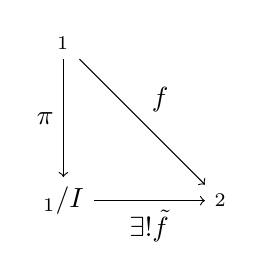
\begin{tikzpicture}[node distance = 2cm]
     \node (g1) {$\g_1$};
     \node (gI) [below of = g1] {$\g_1/I$};
     \node (g2) [right of = gI] {$\g_2$};
     \draw[->] (g1) to node[above right] {$f$} (g2);
     \draw[->] (g1) to node[left] {$\pi$} (gI);
     \draw[->] (gI) to node[below] {$\exists! \tilde{f}$} (g2);
    \end{tikzpicture}
   \end{center}
  \item
   If $I, J \subideal \g$ are subideals with $I \subseteq J$ then $J/I \subideal \g/I$ and the natural isomorphism of vector spaces
   \[
    (\g/I)/(J/I) \to \g/I, \quad (x+I)+(J/I) \mapsto x+I
   \]
   is already a natural isomorphism of Lie algebras.
  \item
   If $I, J \subideal \g$ are subideals then the natural isomorphism of vector spaces
   \begin{gather*}
    (I + J)/J \to I/(I \cap J)
   \shortintertext{defined by}
    (x+J)+I \mapsto x + (I \cap J) \quad \text{for every $x \in I$}
   \end{gather*}
   is already a natural isomorphism of Lie algebras.
 \end{enumerate}
\end{prop}


\begin{rem}
 For a Lie algebra $\g$ the ideal $[\g,\g]$ is the minimal ideal inside $\g$ such that $\g/[\g,\g]$ is abelian. Furthermore given any abelian Lie algebra $\h$ any homomorphism of Lie algebras $\g \to \h$ factorizes through a unique homomorphism of Lie algebras $\g/[\g,\g] \to \h$.
 \begin{center}
  \tikzsetnextfilename{universal_property_of_abelization}
  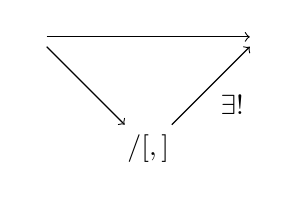
\begin{tikzpicture}[node distance = 2cm]
   \node (gab) {$\g/[\g,\g]$};
   \node (g) [above left of = gab] {$\g$};
   \node (h) [above right of = gab] {$\h$};
   \draw[->] (g) to (h);
   \draw[->] (g) to (gab);
   \draw[->] (gab) to node[below right] {$\exists!$} (h);
  \end{tikzpicture}
 \end{center}
\end{rem}




\subsection{New Lie algebras from old ones}


\begin{defi}
 Let $\g_1$ and $\g_2$ be Lie algebras over the same field $k$. Then the \emph{product} of $\g_1$ and $\g_2$ is defined as the $k$-vector space $\g_1 \times \g_2$ together with the Lie bracket
 \[
  [(x_1, y_1), (x_2, y_2)]
  = ([x_1, x_2], [y_1, y_2])
  \quad
  \text{for all $(x_1, y_1), (x_2, y_2) \in \g_1 \times \g_2$}.
 \]
\end{defi}


\begin{defi}
 Let $\g$ be a Lie algebra and $I \subideal \g$. Then the induced Lie algebra structure on the quotient vector space $\g/I$ is given by
 \[
  [x+I, y+I] = [x,y] + I \quad \text{for all $x,y \in \g$}.
 \]
\end{defi}


\begin{rem}
 The Lie algebra structure on the quotient $\g/I$ is well-defined: If $x,y, x',y' \in \g$ with $x+I = x'+I$ and $y+I = y'+I$ then $x-x' \in I$ and $y-y' \in I$ and thus
 \begin{align*}
  [x,y] + I
  &= [x' + x-x', y' + y-y'] + I \\
  &= [x',y'] + \underbrace{[x', y-y']}_{\in I} + \underbrace{[x-x', y']}_{\in I} + \underbrace{[x-x', y-y']}_{\in I} + I
  = [x', y'] + I.
 \end{align*}
 The additional properties of a Lie bracket follows from the Lie bracket of $\g$ safisfying them.
\end{rem}


\begin{lem}
 \begin{enumerate}[leftmargin=*]
  \item
   If $\g_1$ and $\g_2$ are Lie algebras then the canonical projections
   \[
    \pi_i \colon \g_1 \times \g_2 \to \g_i, \quad (x_1, x_2) \mapsto x_i
    \quad \text{for $i = 1, 2$}
   \]
   are homomorphisms of Lie-algebras.
  \item
   If $\g$ is a Lie algebra and $I \subideal \g$ then the canonical projection $\pi \colon \g \to \g/I, x \mapsto [x]$ is a homomorphism of Lie algebras.
 \end{enumerate}
\end{lem}



\begin{lem}\label{lem: quasi extension of scalars for Lie algebras}
Let $\g$ be a Lie algebra over $k$ and $A$ an associative, commutative $k$-algebra. Then $A \otimes_k \g$ is a Lie algebra over $k$ via
\[
 [a \otimes x, b \otimes y] = (ab) \otimes [x,y]
 \quad
 \text{for all $a,b \in A$ and $x,y \in \g$}.
\]
Similarly $\g \otimes_k A$ carries the structure of a Lie algebra over $k$ via
\[
 [x \otimes a, y \otimes b] = [x,y] \otimes (ab)
 \quad
 \text{for all $x,y \in \g$ and $a,b \in A$}.
\]
\end{lem}


\begin{expl}
 If $L/k$ is a field extension and $\g$ a Lie algebra over $k$, then $L \otimes_k \g$ is a Lie algebra over $k$ via
 \[
  [\lambda \otimes x, \mu \otimes y] = (\lambda \mu) \otimes [x,y]
  \quad
  \text{for alle $\lambda, \mu \in k$ and $x,y \in \g$}.
 \]
 $L \otimes_k \g$ also carries the structure of an $L$-vector space via extension of scalars, i.e.
 \[
  \lambda \cdot (\mu \otimes x) = (\lambda \mu) \otimes x
  \quad
  \text{for alle $\lambda, \mu \in k$ and $x \in \g$},
 \]
 and the Lie bracket is not only $k$-bilinear, but also $L$-bilinear. Hence the structure of a $k$-Lie algebra on $L \otimes_k \g$ can be extended to the structure of a Lie algebra over $L$. (Notice that the Jacobi-Identity is independent of the ground field.)
\end{expl}


\begin{defi}
 Let $\g$ be a Lie algebra and $A = k[t,t^{-1}]$ be the algebra of Laurent polynomials over $k$. Then
 \[
  \Loop(\g) \coloneqq \g \otimes_k A
 \]
 with the Lie bracket as in Lemma~\ref{lem: quasi extension of scalars for Lie algebras} is called the \emph{loop (Lie) algebra} of $\g$.
\end{defi}


Another example for constructing new Lie algebras out of old ones are \emph{central extensions}: Let $\g$ be any $k$-Lie algebra.
\[
 \tilde{\g}
 \coloneqq \g \oplus k
 = \{x + \lambda c \mid x \in \g, \lambda \in k\},
\]
where we understand $c$ as a formal variable. Suppose that $\kappa \colon \g \times \g \to k$ is a $k$-bilinear map satisfying the following properties:
\begin{enumerate}
 \item
  $\kappa$ is antisymmetric, i.e.\ $\kappa(x,y) = -\kappa(y,x)$ for all $x,y \in \g$.
 \item
  $\kappa$ satisfies the $2$-cocycle condition
  \[
   \kappa([x,y],z) + \kappa([y,z],x) + \kappa([z,x],y) = 0
   \quad
   \text{for all $x,y,z \in \g$}.
  \]
\end{enumerate}
Then $\tilde{\g}$ becomes a Lie algebra via
\[
 [x + \lambda c, y + \mu c] \coloneqq [x,y] + \kappa(x,y) \lambda \mu c
 \quad \text{for all $x,y \in \g$ and $\lambda, \mu \in k$.}
\]
Note that $c$ is central in $\tilde{\g}$ in the sense that $[x,c] = 0$ for all $x \in \g$.


\begin{expl}
 Let $\g = \gl_n(k)$. We define a symmetric bilinear form on $\g$ via
 \[
  (A,B)_{\tr} = \tr(AB) \quad \text{for all $A,B \in \g$}.
 \]
 We define a bilinear form
 \[
  \Loop(\g) \times \Loop(\g) \to k[t,t^{-1}], \quad
  (x \otimes p, y \otimes q) \mapsto (x,y)_{\tr}\ pq
 \]
 We now get a $2$-cocycle $\kappa \colon \Loop(\g) \times \Loop(\g) \to k$ via
 \[
  \kappa(a,b) \coloneqq \mathrm{Res}\left(\frac{\partial a}{\partial t}, b\right).
 \]
 $\kappa$ is also antisymmetric: Let $a = x \otimes t^i$ and $b = y \otimes t^j$ with $x,y \in \g$ and $i,j \in \Z$. Then
 \begin{align*}
  \kappa(x \otimes t^i, y \otimes t^j)
  = \mathrm{Res}(i x \otimes t^{i-1}, y \otimes t^j)
  &= \mathrm{Res}(i t^{i+j-1} (x,y)_{\tr}) \\
  &=
  \begin{cases}
   i (x,y)_{\tr} & \text{if $i+j = 0$}, \\
               0 & \text{otherwise}.
  \end{cases}
 \end{align*}
 In the same way we find that
 \[
  \kappa(y \otimes t^j, x \otimes t^i) =
  \begin{cases}
   j (x,y)_{\tr} & \text{if $i+j = 0$}, \\
               0 & \text{otherwise}.
  \end{cases}
 \]
 Since $(\cdot,\cdot)_{\tr}$ is symmetric we find that
 \begin{align*}
  \kappa(x \otimes t^i, y \otimes t^j)
  &=
  \begin{cases}
   i (x,y)_{\tr} & \text{if $i+j = 0$}, \\
               0 & \text{otherwise},
  \end{cases} \\
  &=
  \begin{cases}
   -j (x,y)_{\tr} & \text{if $i+j = 0$}, \\
                0 & \text{otherwise},
  \end{cases} \\
  &=
  -\kappa(y \otimes t^j, x \otimes t^i).
 \end{align*}
\end{expl}





\subsection{Derivations}


\begin{defi}
 Let $A$ be a $k$-algebra (not necessarily unitary of even associative). A \emph{derivation of $A$} is a $k$-linear map $d \colon A \to A$ such that
 \[
  d(ab) = d(a)b + ad(b) \quad \text{for all $a,b \in A$}.
 \]
 We set
 \[
  \Der(A) \coloneqq \{d \colon A \to A \mid \text{$d$ is a derivation of $A$} \}.
 \]
\end{defi}


\begin{rem}
 $\Der(A)$ is a $k$-linear subspace of $\End_k(A)$.
\end{rem}


\begin{expl}
  Let $A$ be a $k$-algebra. It follows from direct calculation that for all $d, d' \in \Der(A)$ the commutator $[d,d'] = d \circ d' - d' \circ d$ is again a derivation $\Der(A)$. Hence $\Der(A)$ is a Lie subalgebra of $\gl(A)$.
\end{expl}


\begin{defi}
 Let $\g$ be a Lie algebra. Then
 \[
  \ad \colon \g \to \gl(\g), \quad x \mapsto [x,\cdot]
 \]
 is called the \emph{adjoint representation} of $\g$.
\end{defi}


\begin{lem}\label{lem: Lie algebras act adjoint by derivations}
 Let $\g$ be a Lie algebra. Then for any $x \in \g$ the map $\ad(x) \colon \g \to \g$ is a derivation of $\g$.
\end{lem}
\begin{proof}
 By the Jacobi identity
 \begin{align*}
  \ad(x)([y,z])
  &= [x,[y,z]]
  = [[x,y],z] + [y,[x,z]] \\
  &= [\ad(x)(y),z] + [y,\ad(x)(z)]
 \end{align*}
 for all $y,z \in \g$.
\end{proof}


\begin{defi}
 Let $\g$ be a Lie algebra. A derivation of $\g$ is called \emph{inner} if it is of the form $\ad(x)$ for some $x \in \g$.
\end{defi}


\begin{lem}
 If $\g$ is a Lie algebra then the inner derivations form an ideal inside of $\Der(\g)$.
\end{lem}
\begin{proof}
 Let $I \coloneqq \im \ad \subseteq \Der(\g)$ be the linear subspace of inner derivations. For any $\delta \in \Der$ and $x \in \g$ it follows that for any $y \in \g$
 \begin{align*}
  &\,[\delta, \ad(x)](y)
  = (\delta \ad(x) - \ad(x) \delta(x))(y) \\
  &= \delta([x,y]) - [x,\delta(y)]
  = [\delta(x),y] + [x,\delta(y)] - [x,\delta(y)] \\
  &= [\delta(x),y]
  = \ad(\delta(x))(y).
 \end{align*}
 Hence $[\delta, \ad(x)] = \ad(\delta(x)) \in I$.
\end{proof}










\subsection{Representations of Lie algebras}



\subsubsection{Definition of a representation}


\begin{defi}
 Let $\g$ be a $k$-Lie algebra. A \emph{representation} of $\g$ is a $k$-vector space $V$ together with a homomorphism of Lie algebras $\rho \colon \g \to \gl(V)$. This representation is called \emph{faithful} if $\rho$ is injective. The \emph{dimension} of this representation is the dimension of $V$.
\end{defi}


\begin{rem}
 Equivalently a representation of $\g$ is a $k$-vector space $V$ together with a $k$-bilinear map $\g \times V \to V, (x,v) \mapsto x.v$ such that
 \[
  x.(y.v) - y.(x.v) = [x,y].v \quad \text{for all $x,y \in \g$ and $v \in V$}.
 \]
 We will not distinguish between these two concepts and choose whichever is more useful in the given situation.
\end{rem}


\begin{defi}
 Let $V$ und $W$ be representations of a $k$-Lie algebra $\g$. A $k$-linear map $f \colon V \to W$ is called a \emph{homomorphism of representations} if
 \[
  f(x.v) = x.f(v) \quad \text{for every $x \in \g$ and $v \in V$}.
 \]
 If $\rho_V \colon \g \to \gl(V)$ and $\rho_W \colon \g \to \gl(W)$ are the corresponding Lie algebra homomomorphisms this is equivalent to
 \[
  f \circ \rho_V(x) = \rho_W(x) \circ f \quad \text{for every $x \in X$}.
 \]
 $f$ is an \emph{isomorphism of representations} if it is additionally bijective.
\end{defi}


\begin{rem}
 If $f \colon V \to W$ is an isomorphism of representations of a Lie algebra $\g$ then the $k$-linear map $f^{-1} \colon W \to V$ is also a homomorphism of representations (and therefore an isomorphism of representations) because
 \[
  f^{-1}(x.v) = f^{-1}(x.f(f^{-1}(v))) = f^{-1}(f(x.f^{-1}(v))) = x.f^{-1}(v)
 \]
 for every $x \in \g$ and $v \in V$. It also follows for every $x \in \g$ from $f \rho_V(x) = \rho_W(x) f$ that $\rho_V(x) f^{-1} = f^{-1} \rho_W(x)$.
\end{rem}





\subsubsection{The adjoint representation}


\begin{expl}
 For any Lie algebra $\g$ the adjoint representation $\ad \colon \g \to \gl(V)$ is a representation of $\g$: That $\ad$ is a homomorphism of Lie algebras is equivalent to
 \begin{gather*}
  \ad([x,y])(z) = [\ad(x),\ad(y)](z) \quad \text{for all $x,y,z \in \g$}.
 \shortintertext{Because}
  \ad([x,y])(z) = [[x,y],z] = -[z,[x,y]]
 \shortintertext{and}
  \begin{aligned}
   [\ad(x),\ad(y)](z)
   &= (\ad(x) \circ \ad(y))(z) - (\ad(y) \circ \ad(x))(z) \\
   &= [x,[y,z]] - [y,[x,z]]
   = [x,[y,z]] + [y,[z,x]]
  \end{aligned}
 \end{gather*}
 this is equivalent to the Jacobi identity. Hence $\ad$ really is a representation of $\g$.
 
 Together with Lemma~\ref{lem: Lie algebras act adjoint by derivations} it follows that $\g$ acts on itself by derivations of itself.

 As $\ker \ad = Z(\g)$ the adjoint representation is faithful if and only if $Z(\g) = 0$.
\end{expl}


\begin{expl}
 If $\g \subseteq \gl(V)$ is a Lie subalgebra then $V$ is a representation of $\g$ via the inclusion $\g \inc \gl(V)$. This corresponds to the action
 \[
  x.v = x(v) \quad \text{for every $x \in \g$ and $v \in V$}.
 \]
\end{expl}



\subsubsection{New representations from old ones}


\begin{prop}
 Let $\g$ be a Lie algebra over a field $k$.
 \begin{enumerate}[leftmargin=*]
  \item
   If $(V_i)_{i \in I}$ is a collection of representations of $\g$ then $\bigoplus_{i \in I} V_i$ is a representation of $\g$ via
   \[
    x.\sum_{i \in I} v_i = \sum_{i \in I} x.v_i
   \]
   or every $x \in \g$ and $v_i \in V_i$ for all $i \in I$, with $v_i = 0$ for all but finitely many $i \in I$.
  \item
   If $V$ and $W$ are representations of $\g$ then $V \otimes W$ is a representation of $\g$ via
   \[
    x.(v \otimes w) = (x.v) \otimes w + v \otimes (x.w) \quad \text{for every $x \in \g$, $v \in V$ and $w \in W$}.
   \]
   More generally: If $V_1, \dotsc V_n$ are representations of $\g$ then $\bigotimes_{i=1}^n V_i$ is a representation of $\g$ via
   \[
    x.(v_1 \otimes \dotsb \otimes v_n)
    = \sum_{i=1}^n v_1 \otimes \dotsb \otimes v_{i-1} \otimes (x.v_i) \otimes v_{i+1} \otimes \dotsb \otimes v_n.
   \]
   for every $x \in \g$ and $v_i \in V_i$ for every $i = 1, \dotsc, n$.
  \item
   If $V, W$ are representations of $V$ then $\Hom_k(V,W)$ is a representation of $\g$ via
   \[
    (x.f)(v) = x.f(v) - f(x.v) \quad \text{for every $x \in \g$, $f \in \Hom(V,W)$ and $v \in V$}.
   \]
  \item
   By letting $\g$ act trivially on $k$ the dual $V^* = \Hom_k(V,k)$ becomes a representation of $\g$ in the above way, i.e.
   \[
    (x.\varphi)(v) = -\varphi(x.v) \quad \text{for every $x \in \g$, $\varphi \in V^*$ and $v \in V$}.
   \]
 \end{enumerate}
\end{prop}


\begin{prop}
 Let $\g$ be a Lie algebra.
 \begin{enumerate}[leftmargin=*]
  \item
   If $V$ and $W$ are finite dimensional representations of $\g$ then the map
   \[
    V^* \otimes W \to \Hom_k(V,W), \quad \varphi \otimes w \mapsto (v \mapsto \varphi(v) w)
   \]
   is a homomorphism of representations. If $V$ and $W$ are both finite dimensional this is an isomorphism of vector spaces and thus already an isomorphism of representations.
  \item
   If $V^i_j$ with $i = 1, \dotsc, r$ and $j = 1, \dotsc, n_i$ is a collection of representations of $\g$ then the isomorphism of vector spaces
   \begin{align*}
    \bigotimes_{i=1}^r \bigotimes_{j=1}^{n_j} V^{i}_j
    &\to V^1_1 \otimes \dotsb \otimes V^1_{n_1} \otimes \dotsb \otimes V^r_1 \otimes \dotsb \otimes V^{r}_{n_r}, \\
    (v^1_1 \otimes \dotsb \otimes v^1_{n_1}) \otimes \dotsb \otimes (v^r_1 \otimes \dotsb \otimes v^r_{n_r})
    &\mapsto v^1_1 \otimes \dotsb \otimes v^1_{n_1} \otimes \dotsb \otimes v^r_1 \otimes \dotsb \otimes v^r_{n_r}
   \end{align*}
   is already an isomorphism of representations.
  \item
   If $V_1, \dotsc, V_n$ and $W_1, \dotsc, W_n$ are representations of $\g$ and $f_i \colon V_i \to W_i$ for every $i = 1, \dotsc, n$ a homomorphism of representations it follows that the map
   \[
    f_1 \otimes \dotsb \otimes f_n \colon \bigotimes_{i=1}^n V_i \to \bigotimes_{i=1}^n W_i,
    v_1 \otimes \dotsb \otimes v_n \mapsto f(v_1) \otimes \dotsb \otimes f(v_n)
   \]
   is also a homomorphism of representations.
 \end{enumerate}
\end{prop}


\subsubsection{Subrepresentations and irreducible representations}


\begin{defi}
 Let $\g$ be a Lie algebra and $\rho \colon \g \to \gl(V)$ a representation of $\g$. A \emph{subrepresentation} of $V$ is a linear subpace $U \subseteq V$ such that $x.u \in U$ for every $x \in \g$ and $u \in U$. Equivalently $U$ is $\rho(x)$ invariant for every $x \in \g$.
 
 If $(U_i)_{i \in I}$ is a collection of subrepresentations of $\g$ then $V$ is called the \emph{direct sum} of the $U_i$ if $V = \bigoplus_{i \in I} U_i$ as vector spaces.
\end{defi}


\begin{expls}
 Let $\g$ be a Lie algebra.
 \begin{enumerate}[leftmargin=*]
  \item
   If $V$ is a representation of $\g$ then $0$ and $V$ itself are subrepresentations. These are also called the \emph{trivial subrepresentations}.
  \item
   If $V$ is a representation and $(U_i)_{i \in I}$ a collection of subrepresentations $U_i \subseteq V_i$ then $\sum_{i \in I} U_i$ is also a subrepresentation of $V$.
  \item
   The subrepresentations of the adjoint representation of $\g$ are precisely the ideals in $\g$.
 \end{enumerate}
\end{expls}


\begin{defi}
 A representation $V$ of a Lie algebra $\g$ is called \emph{irreducible} if it has precisely two subrepresentations. Equivalently $V$ is nonzero and has only the trivial subrepresentations.
 
 $V$ is called \emph{decomposable} if there exist non-trivial subrepresentations $U_1, U_2 \subseteq V$ with $V = U_1 \oplus U_2$. Otherwise $V$ is called \emph{indecomposable}.
\end{defi}


\begin{rem}
 By definition every irreducible representation is also indecomposable. The converse does not hold.
\end{rem}



\begin{expl}
 The adjoint representation of a Lie algebra $\g$ is irreducible if and only if $\g \neq 0$ and $\g$ has no ideals besides $0$ and $\g$ itself. So $\g$ is either the onedimensional abelian Lie algebra or a simple Lie algebra.
\end{expl}







\subsection{Simple Lie algebras}


\begin{defi}
 A Lie algebra $\g$ is \emph{simple} if $0$ and $\g$ are the only ideals inside $\g$ and $\g$ is not abelian.
\end{defi}


\begin{lem}
 Let $\g$ be a simple Lie algebra. Then $[\g,\g] = \g$ and $Z(\g)=0$.
\end{lem}
\begin{proof}
 Because $\g$ is simple it is not abelian. Therefore $[\g,\g] \neq 0$ and $Z(\g) \neq \g$. Since $[\g,\g]$ and $Z(\g)$ are ideals inside $\g$ it follows that $[\g,\g] = \g$ and $Z(\g) = 0$.
\end{proof}


\begin{cor}
 Let $\g$ be simple. Then $\ad \colon \g \to \gl(\g)$ is injective. In particular $\g$ can be realized as a linear Lie algebra.
\end{cor}
\begin{proof}
 This directly follows from $\ker \ad = Z(\g) = 0$.
\end{proof}


It can be shown that every finite dimensional Lie algebra can be realized as a linear Lie algebra. This will not be proven in this lecture and is by far not trivial.


\begin{thrm}[Ado]
 Every finite dimensional Lie algebra $\g$ is isomorphic to a linear Lie algebra (which is equivalent to $\g$ having a faithful finite-dimensional representation).
\end{thrm}


\begin{expls}
 \begin{enumerate}[leftmargin=*]
  \item
   Since $[\gl_n(k),\gl_n(k)] = \sll_n(k) \neq \gl_n(k)$ we find that $\gl_n(k)$ is not simple.
  \item
   Let $\g = \sll_2(k)$. Then $\g$ is simple if and only if $\chara k \neq 2$. To see this consider the basis $(e,h,f)$ of $\sll_2(k)$ consisting of the matrices
   \[
    e = \begin{pmatrix}0 & 1 \\ 0 & 0\end{pmatrix}, \quad
    h = \vect{1 & 0 \\ 0 & -1}, \quad
    f = \vect{0 & 0 \\ 1 & 0}.
   \]
   of $\sll_2(k)$. Then
   \[
    [h,e] = 2e, \quad
    [h,f] = -2f, \quad
    [e,f] = h.
   \]
   If $\chara k = 2$ then $h$ spans a $1$-dimensional ideal, thus $\sll_2(k)$ is not simple. Suppose that $\chara k \neq 2$ and let $I \subseteq \sll_2(k)$ be an ideal with $I \neq 0$. It is clear that if $I$ contains one of the basis vectors $e$, $h$ or $f$ it follows that $I = \sll_2(k)$. Let $x \in I$ with $x \neq 0$ and write $x = \alpha e + \beta h + \gamma f$. Then
   \[
    [e,x] = -2 \beta e + \gamma h \quad \text{and} \quad [e,[e,x]] = -2 \gamma e.
   \]
   Since $\gamma = 0$ or $\gamma \neq 0$ we find that $e \in I$.
 \end{enumerate}
\end{expls}


\begin{rem}
 If $\chara k = 0$ then $\sll_n(k)$ is simple for all $n \geq 2$.
\end{rem}